\begin{frame}{Test}
\framesubtitle{Setup}
\begin{columns}
\begin{column}{0.5\textwidth}

\begin{figure}[H]
    \centering
    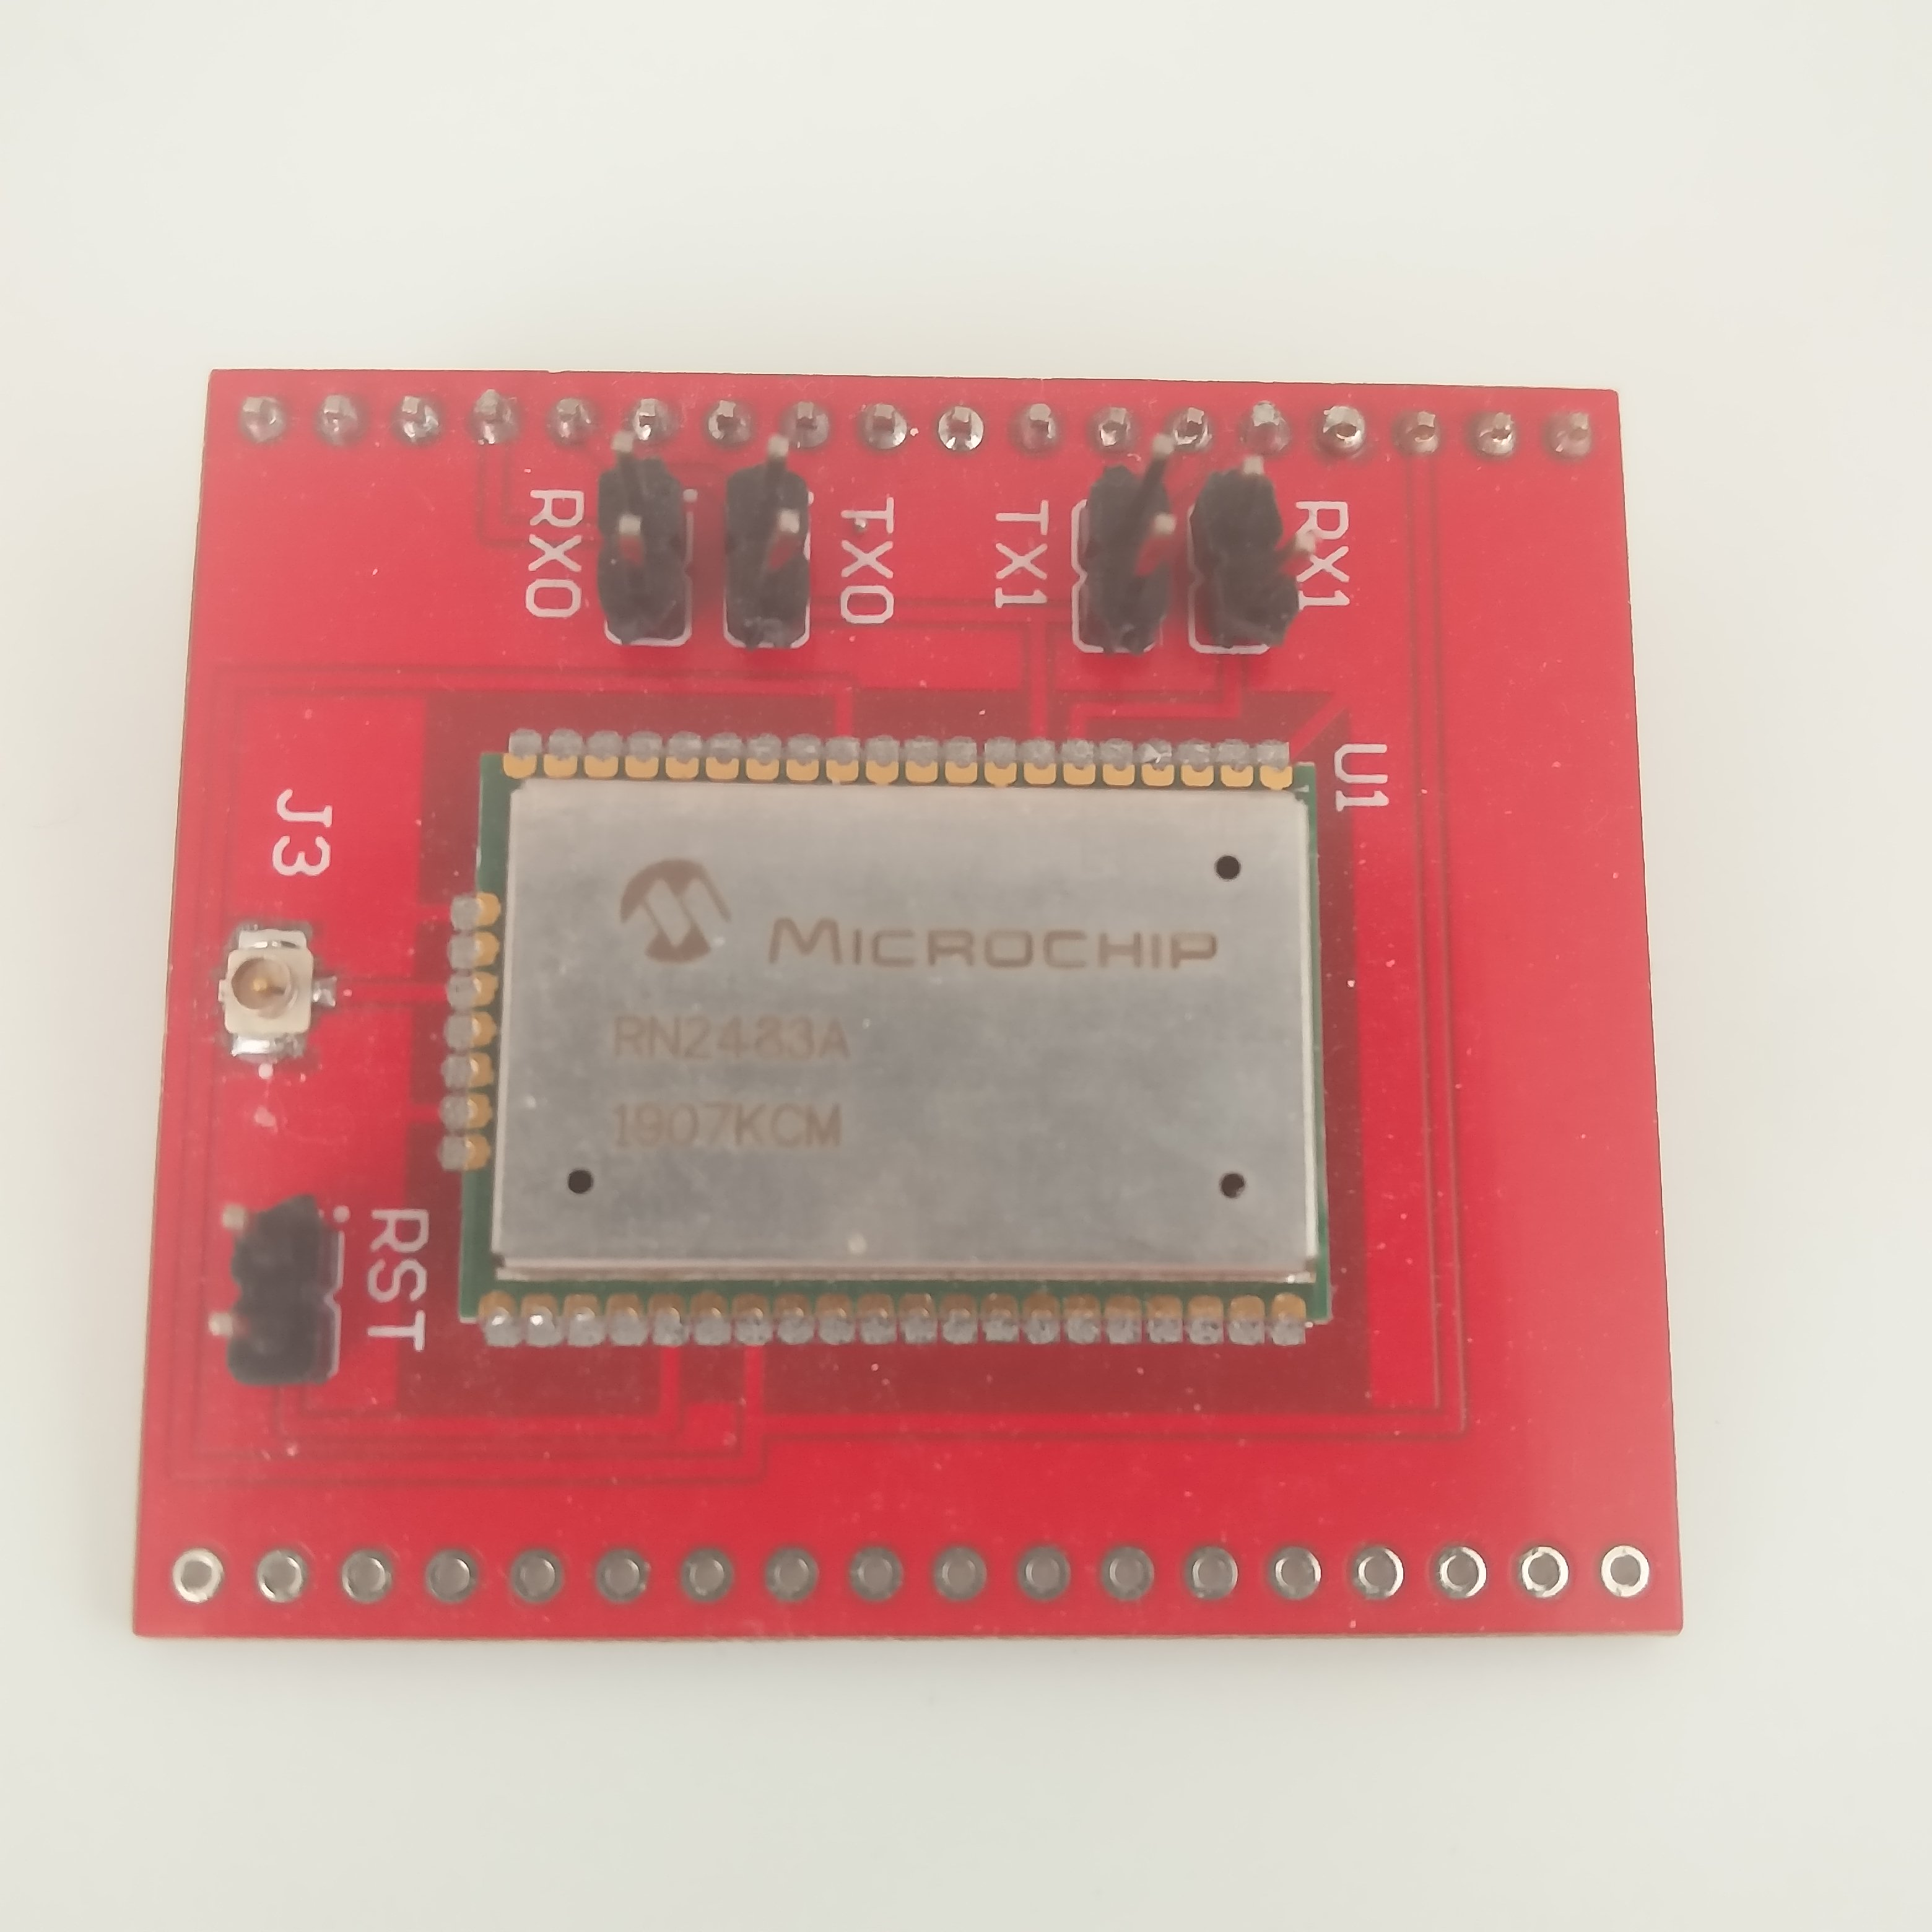
\includegraphics[width=0.6\textwidth]{presentation.tex/fig/rn2483.jpg}
    \caption{The RN2483 LoRa radio shield\label{fig:rn2483pic}}
\end{figure}
\end{column}
\begin{column}{0.5\textwidth}
\begin{figure}[H]
    \centering
    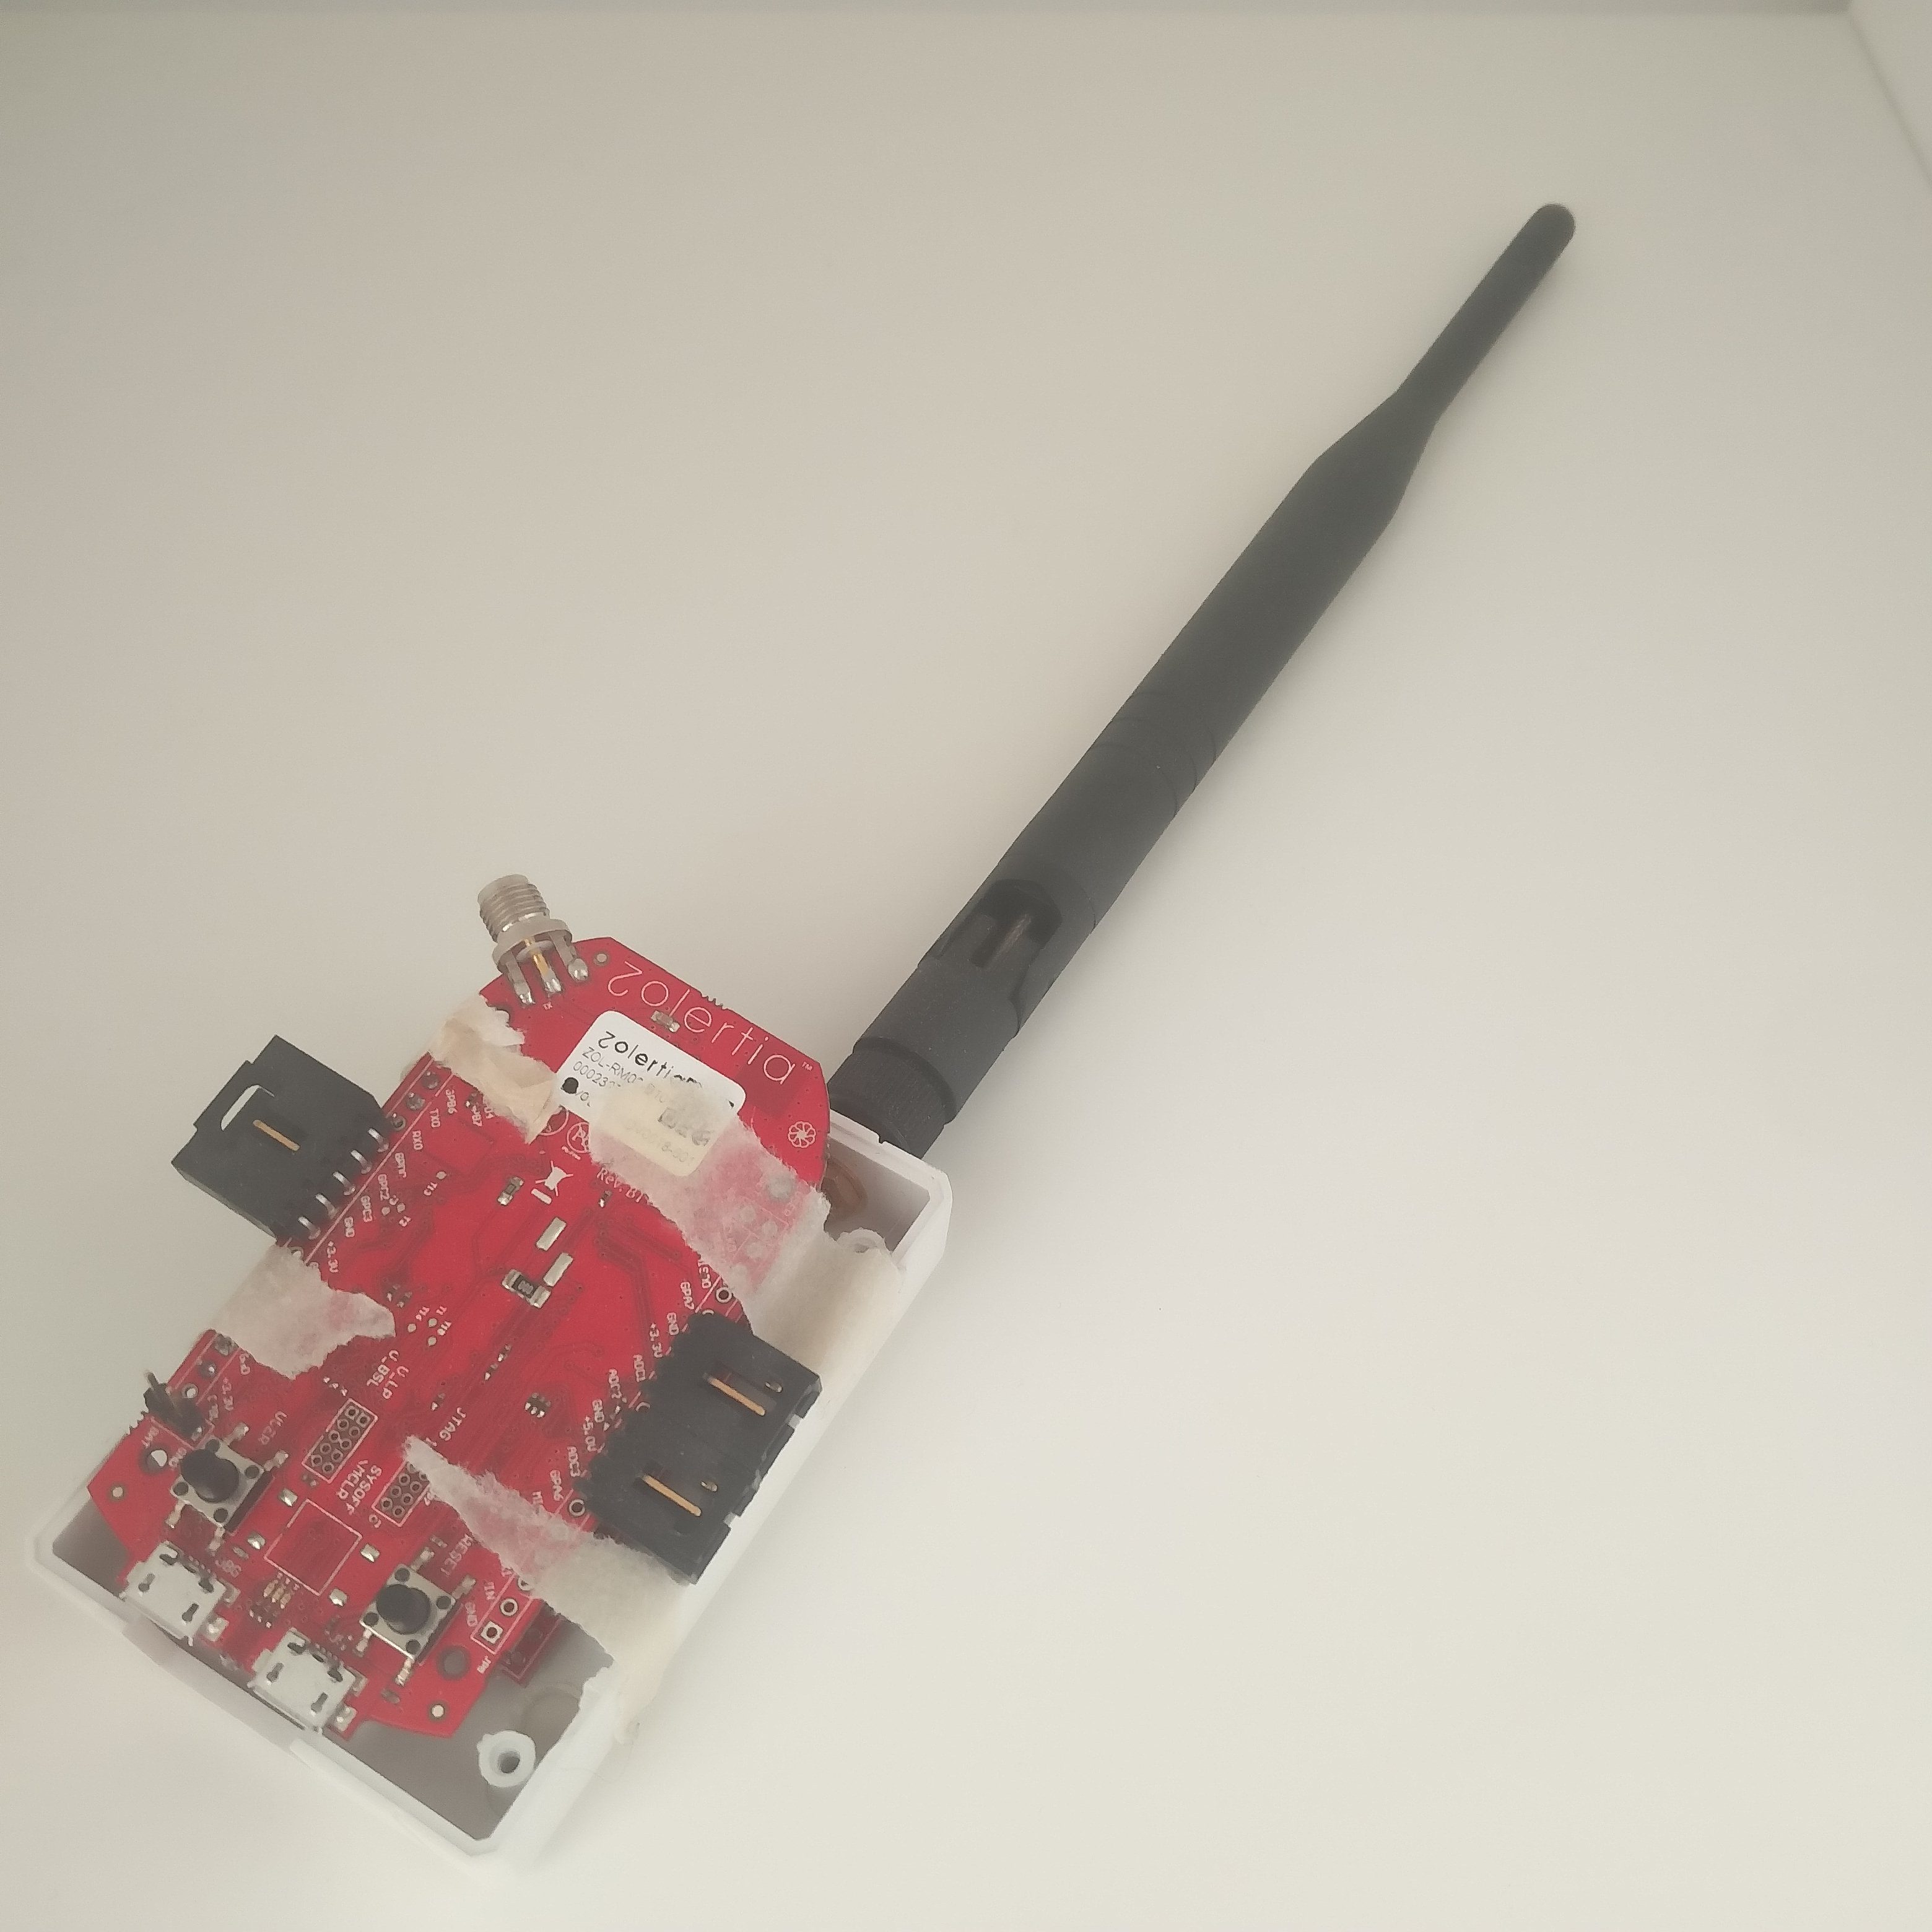
\includegraphics[width=0.6\textwidth]{presentation.tex/fig/zolertia.jpg}
    \caption{The Zolertia RE-Mote with the shield\label{fig:zolpic}}
\end{figure}
\end{column}
\end{columns}
\end{frame}

\begin{frame}{Test}
\framesubtitle{Driver}

\begin{columns}
\begin{column}{0.5\textwidth}

\end{column}
\begin{column}{0.5\textwidth}

\end{column}
\end{columns}

\end{frame}

\begin{frame}{Test}
\framesubtitle{Adapt TSCH for LoRa}
\begin{columns}
\begin{column}{0.5\textwidth}
\begin{itemize}
    \item Time slot parts timing 
    \item Adaptation to 64bits
    \item Interrupt clash
    \item Watchdog
\end{itemize}
\end{column}
\begin{column}{0.5\textwidth}
\end{column}
\end{columns}
\end{frame}

\begin{frame}{Test}
\framesubtitle{Adapt TSCH for LoRa}
\begin{columns}
\begin{column}{0.5\textwidth}
\begin{itemize}
    \item Physical delay of RN2483
    \item Drift Issues
\end{itemize}
\end{column}
\begin{column}{0.5\textwidth}
\end{column}
\end{columns}
\end{frame}

\begin{frame}{Test}
\framesubtitle{RPL}
\begin{figure}[H]
    \centering
    \resizebox{8.5cm}{4.5cm}{%
  \begin{tikzpicture}[]

  \begin{scope}[
      xshift=-0.2cm,
      asn/.style={black!70, minimum width=2cm},
      timeslot/.style={draw, rectangle, minimum width=2cm, minimum height=1cm},
      arr/.style={help lines,black!70,<->},
  ]
    \foreach \i in {0,...,7} {
      \node (ts\i) [asn] at (2*\i, 1) {$TS_{\i}$};
    }
    \node (tss0) [timeslot] at (0, 0) {\tiny Shared};
    \node (tss1) [timeslot] at (2, 0) {\tiny :2dac $\rightarrow$ :2f2a};
    \node (tss2) [timeslot] at (4, 0) {\tiny :2dbc $\rightarrow$ :2f2a};
    \node (tss3) [timeslot] at (6, 0) {\tiny :2dbc $\rightarrow$ :2dac};
    \node (tss4) [timeslot] at (8, 0) {\tiny :2f2a $\rightarrow$ :2dbc};
    \node (tss5) [timeslot] at (10, 0) {\tiny :2f09 $\rightarrow$ :2dac};
    \node (tss6) [timeslot] at (12, 0) {\tiny :2dac $\rightarrow$ :2f09};
    \node (tss7) [timeslot, fill=black!30] at (14, 0) {};
  \end{scope}
  \begin{scope}[xshift=5cm,yshift=-2cm,->,>=stealth',shorten >=1pt,auto,node distance=2.5cm]
    \tikzstyle{every state}=[thick,draw=gray!50,fill=gray!20,draw=none,text=black]

    \node[state,thick,draw=red!40]         (A) [] {:2f2a};
    \node[state]         (B) [below of=A]       {:2dac};
    \node[state]         (C) [right of=B]       {:2dbc};
    \node[state]         (D) [left of=B]       {:2f09};

    \path (A) edge [bend left] node {$TS_4$} (C)
          (B) edge [bend left] node {$TS_1$} (A)
              edge [bend left] node {$TS_6$} (D)
          (C) edge [bend left] node[above right] {$TS_2$} (A)
              edge [bend left] node {$TS_3$} (B)
          (D) edge [bend left] node {$TS_5$} (B);
  \end{scope}
\end{tikzpicture}
}
\caption{Custom Schedule\label{fig:customsched}}
\end{figure}
\end{frame}

\begin{frame}{Test}
\framesubtitle{Jamming}
\begin{figure}[H]
\centering

\begin{tikzpicture}[auto, node distance=2cm,>=latex']

\tikzset{
  block/.style = {draw, fill=white, rectangle, minimum height=3em, minimum width=2cm},
  input/.style = {coordinate},
  output/.style = {coordinate},
  pinstyle/.style = {pin edge={to-,t,black}},
  radiation/.style={decorate,decoration={expanding waves,angle=12,segment length=4pt}},
  zigzag/.style={to path={ -- ($(\tikztostart)!.55!-7:(\tikztotarget)$) -- ($(\tikztostart)!.45!7:(\tikztotarget)$) -- (\tikztotarget) \tikztonodes}}
}
\node[block](tx){Transmitter Node};
\node[block,above right= 2cm of tx](ttx){Jammer};
\node[block,right = 5cm of tx](rx){Coordinator Node};

\draw[radiation] ([shift={(1cm,0cm)}]tx.east)-- node [above=5mm] {} ([shift={(-1cm,0cm)}]rx.west);
\draw[-stealth,line width=1mm] (ttx.south) to[zigzag] +(0,-1.5);
\end{tikzpicture}

\caption{Structure of the channel jamming test\label{fig:jammer}}
\end{figure}
\end{frame}

\begin{frame}{Test}
\framesubtitle{Jamming}
\begin{figure}[H]
  \centering
  \begin{tikzpicture}

  \begin{groupplot}[group style={group size=1 by 2,
      horizontal sep=0pt,
      vertical sep=1cm},
      height=6cm,width=6cm,
  ]
  \nextgroupplot[
    ycomb,
    width=0.8\textwidth,
    height=0.25\textwidth,
    axis lines=middle,
    ymin=0,
    ymax=4,
    ylabel={$Retry_{number}$},
    ylabel near ticks,
    yticklabel style={/pgf/number format/1000 sep=},
    xmin=0,
    xmax=50,
    xlabel={$Transmission_{number}$},
    xlabel near ticks,
  ]
    \addplot[color=blue, mark=x] coordinates {
      (1,1)
      (2,2)
      (3,0)
      (4,0)
      (5,0)
      (6,1)
      (7,0)
      (8,0)
      (9,1)
      (10,0)
      (11,1)
      (12,1)
      (13,2)
      (14,0)
      (15,2)
      (16,0)
      (17,1)
      (18,1)
      (19,1)
      (20,0)
      (21,4)
      (22,0)
      (23,0)
      (24,1)
      (25,0)
      (26,0)
      (27,2)
      (28,1)
      (29,0)
      (30,0)
      (31,1)
      (32,1)
      (33,0)
      (34,0)
      (35,0)
      (36,1)
      (37,2)
      (38,0)
      (39,0)
      (40,0)
      (41,1)
      (42,1)
      (43,0)
      (44,0)
      (45,3)
      (46,1)
      (47,0)
      (48,0)
      (49,1)
      (50,1)
    };
  \end{groupplot}
  \end{tikzpicture}
  \caption{Retransmission per packet\label{fig:retransmission}}
\end{figure}
\end{frame}
